\documentclass{beamer}
\usetheme{CMU}

\usepackage{pgf,pgfarrows,pgfnodes,pgfautomata,pgfheaps,pgfshade}
\usepackage{amsmath,amssymb}
\usepackage[utf8]{inputenc}
\usepackage{colortbl}
\usepackage[english]{babel}
\usepackage{booktabs}
\usepackage{slpython}
\usepackage{underscore}

\author{Luís Pedro Coelho}
\institute{Programming for Scientists}

\graphicspath{{figures/}{figures/generated/}{images/}}

\newcommand*{\code}[1]{\textsl{#1}}


\title{Numerical Representations}
\begin{document}
\frame{\maketitle}

\begin{frame}[fragile]
\frametitle{How Are Numbers Represented}

It's all 0s \& 1s. How do you represent 123?

\end{frame}

\begin{frame}[fragile]
\frametitle{Binary Notation}

$(b_4b_3b_2b_1b_0)_2 = b_4 2^4 + b_3 2^3 + b_2 2^2 + b_1 2^1 + b_0 2^0 = 16b_4 + 8b_3 + 4b_2 + 2 b_1 + b_0$

\end{frame}

\begin{frame}[fragile]
\frametitle{Common Number Sizes}

\begin{itemize}
\item Byte: 8 bits, 0 to 255 ($2^8-1$).
\item Short: 16 bits, 0 to 65535 ($2^{16}-1$).
\item 32-bit int: 32 bits, 0 to 4294967295 ($2^{32}-1$).
\item 64-bit int: 64 bits, 0 to 18446744073709551615 ($2^{64}-1$).
\end{itemize}
\end{frame}

\begin{frame}[fragile]
\frametitle{Bit-wise operations}

\begin{enumerate}
\item NOT(A): true if A is \alert{not} true (\lstinline{~A})
\item AND(A,B): true if A is true and B is true (\lstinline{A & B})
\item OR(A,B): true if either A or B are true (\lstinline{A | B})
\item XOR(A,B): true if one is true and the other is false \lstinline{A ^ B}
\end{enumerate}

\note{
    Two ways to view a number: as a number or as a collection of bits.
}
\end{frame}

\begin{frame}[fragile]
\begin{python}
def fact(N):
     if N == 0: return 1
     return N * fact(N-1)

print  fact(100)
\end{python}

Prints out

933262154439441526816992388562667004907159682643816214\\
685929638952175999932299156089414639761565182862536979\\
20827223758251185210916864000000000000000000000000L

\end{frame}

\begin{frame}[fragile]

What about negative numbers?

\end{frame}

\begin{frame}[fragile]

\begin{itemize}
\item Sign bit
\item Biasing
\item Ones' complement
\item Twos' complement
\end{itemize}
\end{frame}

\begin{frame}[fragile]
\frametitle{Sign Bit}

$(s b_4 b_3 b_2 b_1 b_0)_2 = (-1)^s \left(b_4 2^4 + b_3 2^3 + b_2 2^2 + b_1 2^1 + b_0 2^0 \right)$

\end{frame}

\begin{frame}[fragile]
\frametitle{Biasing}

Have a bias $B$, so that the number $n$ is representated as unsigned$(n+B)$.

\end{frame}

\begin{frame}[fragile]
\frametitle{One's Complement}

If $(b_k b_{k-1}\cdots b_1 b_0)_2$ is some number $n$, then we represent $-n$ by\\
$(\tilde{}b_k \tilde{}b_{k-1}\cdots \tilde{} b_1 \tilde{} b_0)_2$ is some number $n$, then we represent $-n$ by

\pause

\bigskip
$(00000011)_2$ is $\phantom{-}3$\\
$(11111100)_2$ is $-3$

\bigskip

$(00001111)_2$ is $\phantom{-}31$\\
$(11110000)_2$ is $-31$

\bigskip

\pause
$(00000000)_2$ is $\phantom{-}0$\\
$(11111111)_2$ is $-0$

\pause
\bigskip

Ones' complement is not actually used in any modern machine.

\end{frame}

\begin{frame}[fragile]
\frametitle{Twos' Complement}

\centering
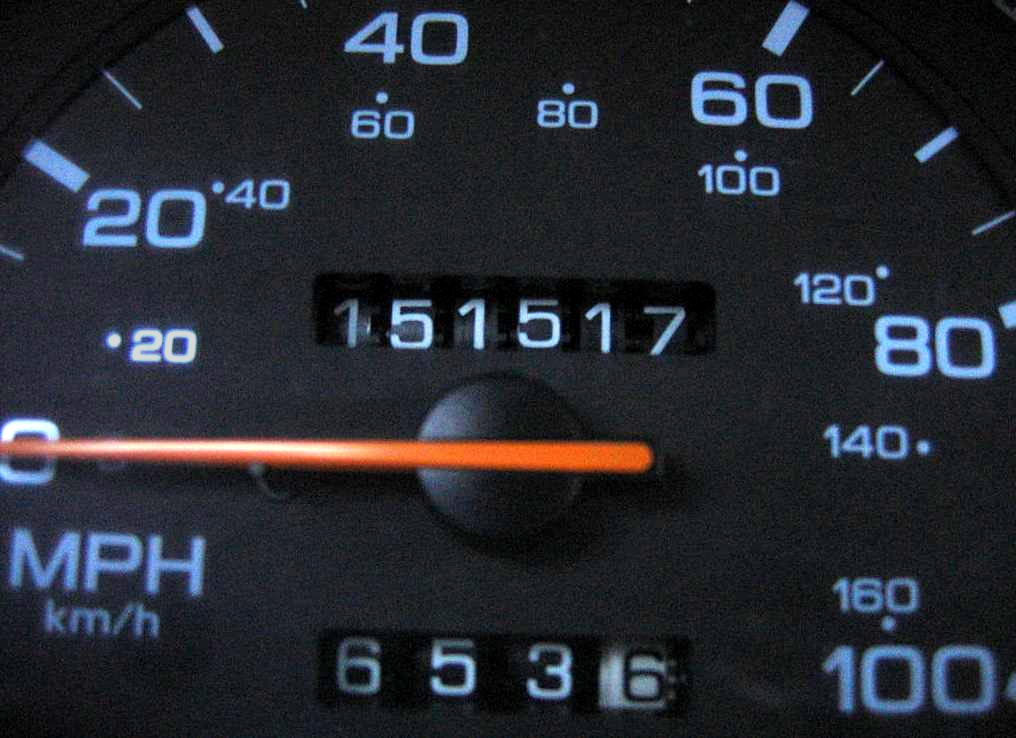
\includegraphics[width=.7\textwidth]{Odometer2.jpg}

\begin{flushright}
Image from Wikipedia\\
Metaphor from Steve Heller
\end{flushright}
\end{frame}

\begin{frame}[fragile]
\frametitle{Twos' Complement}

$(11111111)_2$ is $-1$

$(11111110)_2$ is $-2$

$(11111101)_2$ is $-3$

\note{
    Show addition/subtraction of 2s complement.

    Note that we do have a sign bit.
}
\end{frame}

\begin{frame}[fragile]
\frametitle{Ranges}

\begin{itemize}
\item 8 bits: $-128$ to $127$.
\item 16 bits: $-32768$ to $32767$.
\item 32 bits: $-2147483648$ to $2147483647$.
\item 64 bits: $-9223372036854775808$ to $9223372036854775807$.
\end{itemize}
\end{frame}

\begin{frame}[fragile]
\frametitle{Fractional Numbers}

What about fractional numbers?

\begin{itemize}
\item Fixed point
\item Floating point
\end{itemize}

\end{frame}

\begin{frame}[fragile]
\frametitle{Fixed Point}

Given a fixed base $B$, then an integer $n$ really represents the number $n * 2^B$.

\note{
    Mention how this is used for money.
}

\end{frame}

\begin{frame}[fragile]
\frametitle{Floating Point}

$602214179303030303030303$

\pause
$6.022 * 10^{23}$
\note{
    This is Avogadro's Number.
}
\end{frame}

\begin{frame}[fragile]
\frametitle{Floating Point Representation}

\[
(-1)^s * c * 2^q
\]

\centering
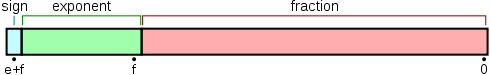
\includegraphics[width=.6\textwidth]{images/FP-format.png}

\note{
    Image (as all images in this lecture) from Wikipedia
}
\end{frame}

\begin{frame}[fragile]
\frametitle{IEEE-754}

\centering
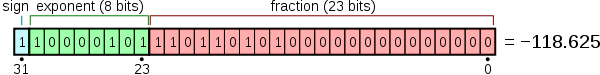
\includegraphics[width=.8\textwidth]{images/FP-example.png}

\end{frame}

\begin{frame}[fragile]
\frametitle{IEEE-754 Formats}

\begin{itemize}
\item 32-bit floats: 1 sign bit, 23 bit fraction, 8 bit exponent.
\item 64-bit floats: 1 sign bit, 52 bit fraction, 11 bit exponent.
\item \alert{Non-standard} 80-bit floats: 1 sign bit, 64 bit fraction, 15 bit exponent.
\end{itemize}
\end{frame}

\begin{frame}[fragile]
\frametitle{Ranges}

\begin{itemize}
\item 32-bit float: $\pm 1.18 10^{-38}$ to $\pm 3.4 10^{38}$.
\item 64-bit float: $\pm 2 10^{-308}$ to $\pm 1.8 ^{308}$.
\end{itemize}
\end{frame}

\begin{frame}[fragile]
\frametitle{Limited Precision}

\begin{python}

print 0.3 * 3
print (0.3 * 3) == .9
\end{python}
prints
\begin{verbatim}
.9
False
\end{verbatim}
\end{frame}

\begin{frame}[fragile]
\begin{python}
print 1.1 * 0 == 0.0  
print 1.1 * 1 == 1.1  
print 1.1 * 2 == 2.2 
print 1.1 * 3 == 3.3 
print 1.1 * 4 == 4.4 
print 1.1 * 5 == 5.5 
print 1.1 * 6 == 6.6 
print 1.1 * 7 == 7.7 
print 1.1 * 8 == 8.8 
print 1.1 * 9 == 9.9 
print 1.1 *10 == 11 
\end{python}
\end{frame}

\begin{frame}[fragile]
\begin{python}
print 1.1 * 0 == 0.0    #  True
print 1.1 * 1 == 1.1    #  True
print 1.1 * 2 == 2.2    #  True
print 1.1 * 3 == 3.3    #  False
print 1.1 * 4 == 4.4    #  True
print 1.1 * 5 == 5.5    #  True
print 1.1 * 6 == 6.6    #  False
print 1.1 * 7 == 7.7    #  False
print 1.1 * 8 == 8.8    #  True
print 1.1 * 9 == 9.9    #  True
print 1.1 *10 == 11     #  True
\end{python}
\end{frame}

\begin{frame}[fragile]
You never compare two floating-point numbers for equality!
\end{frame}

\begin{frame}[fragile]

\begin{python}
x = 0.0
while x < big_number:
    ... # x is unchanged in here!
    x += 1.
\end{python}

Can this go into an infinite loop?

\pause
Yes, it can!
\end{frame}

\begin{frame}[fragile]
\frametitle{Overflow \& Underflow}

When numbers are too big, we say they \alert{overflow}.

When they are too small, we say they \alert{underflow}.
\end{frame}


\begin{frame}[fragile]
\frametitle{Catastrophic Cancellation}

\[
\lim_{x \to 0} \frac{1-\cos x}{x^2}
\]

\note{
    work out on blackboard using Taylor expansion:

    cos x = 1 - x2/2! + x4/4! - x6/6! + \ldots

}%
\begin{flushright}
(Example from ``Introduction to Programming in Java'')
\end{flushright}
\note{http://www.cs.princeton.edu/introcs/home/}
\end{frame}
\begin{frame}[fragile]
\frametitle{Catastrophic Cancellation}

\centering
\includegraphics[width=.9\textwidth]{catastrophic.pdf}

\end{frame}

\begin{frame}[fragile]
\frametitle{Be Careful}

\begin{itemize}
\item Use existing implementations of algorithms instead of rolling your own.
\item Don't trust your instincts.
\end{itemize}
\end{frame}

\begin{frame}[fragile]
\frametitle{Some Special Numbers}

\begin{itemize}
\item $-0$: minus zero.
\item $\pm \infty$
\item NaN: Not a Number
\end{itemize}
\end{frame}

\begin{frame}[fragile]
\frametitle{NaN}
\begin{python}
A = float('NaN')

print A == A
\end{python}
prints \alert{False}!!

\end{frame}

\end{document}
